%==============================================================================
%  CENG493 — Final Report
%  Turkish Legal RAG. IEEE conference (two-column) format.
%  Compile with pdfLaTeX on Overleaf (utf8 + T1 handle Turkish glyphs).
%==============================================================================
\documentclass[conference]{IEEEtran}
\IEEEoverridecommandlockouts

\usepackage[utf8]{inputenc}
\usepackage[T1]{fontenc}
\usepackage{lmodern}
\usepackage{amsmath,amssymb}
\usepackage{graphicx}
\usepackage{booktabs}
\usepackage{array}
\usepackage{multirow}
\usepackage{xcolor}
\usepackage{url}
\usepackage[hidelinks]{hyperref}
\usepackage{tikz}
\usetikzlibrary{arrows.meta,positioning,fit,backgrounds}

% Compact table font
\newcommand{\tnote}[1]{{\footnotesize #1}}
\newcommand{\best}[1]{\textbf{#1}}
\newcommand{\good}{\textcolor{green!55!black}{$\uparrow$}}
\newcommand{\bad}{\textcolor{red!70!black}{$\downarrow$}}

\begin{document}

\title{Improving Turkish Legal Question Answering with a\\
Triage-Driven Retrieval-Augmented Generation Pipeline}

\author{
\IEEEauthorblockN{Berkay Akta\c{s} \quad Arzu Tu\u{g}\c{c}e Koca \quad \c{S}ahin Er\c{s}an}
\IEEEauthorblockA{CENG493 --- Department of Computer Engineering\\
\texttt{github.com/berkay-aktas/hukuk-rag}}
}

\maketitle

\begin{abstract}
We present a domain-adapted retrieval-augmented generation (RAG) system for
Turkish legal question answering, and a controlled ablation that inverts a
common assumption about where adaptation pays off. Starting from a naive hybrid
baseline (Token~F1 $0.1411$), we evaluate three independent fine-tuning
interventions---a contrastively adapted dense encoder, a domain-tuned
cross-encoder reranker, and a QLoRA-tuned generator---against a $225$-question
gold set verified against official statute text. A failure-mode triage
performed \emph{before} spending compute reveals that generation, not
retrieval, is the dominant bottleneck; and the ablation shows that
\emph{only} embedding fine-tuning helps, while our fine-tuned reranker and
single-passage QLoRA both \emph{degrade} end-to-end accuracy. The decisive
gains instead come from (i)~an off-the-shelf Turkish reranker, (ii)~a
source-filtered verbatim-snap post-processor, and (iii)~scaling the generator
from 7B to 14B parameters---together lifting Token~F1 to \best{$0.2648$}
($+87.7\%$ over baseline), BERTScore~F1 to $0.716$, and an LLM-judged
correctness of $0.75$ (validated against an independent Claude judge,
Spearman~$\rho{=}0.72$, $p{<}0.001$), while roughly halving the hallucination
rate ($17.0\%\rightarrow 8.95\%$). Production retrieval attains Recall@10
$0.875$ on a chunk-labeled benchmark. We characterize each failed intervention
as a transferable negative result---silver-label noise, a single-passage /
multi-passage format mismatch that paradoxically lifts faithfulness $+24$pp
while lowering Token~F1, and a generator domain-knowledge gap that breaks
HyDE---and ship an evaluator-agnostic pipeline that runs the full
Recall\,+\,F1\,+\,Faithfulness suite on arbitrary user-supplied documents.
\end{abstract}

\begin{IEEEkeywords}
retrieval-augmented generation, Turkish NLP, legal NLP, cross-encoder
reranking, QLoRA, hallucination, ablation study, negative results.
\end{IEEEkeywords}

%==============================================================================
\section{Introduction}
%==============================================================================
Turkish legal question answering (QA) stresses every stage of a RAG pipeline.
Retrieval must contend with agglutinative morphology---a single verb can encode
tense, person, negation, and modality, yielding thousands of surface forms per
lemma---and with locale-specific casing (the capital ``I'' maps to dotless
``\i''), so a naive pipeline mis-tokenizes both queries and documents.
Generation must produce \emph{grounded} answers that cite specific provisions
(e.g., ``\emph{5237 say\i l\i\ TCK Madde~81}'') while minimizing
hallucination---a consequential failure mode in a legal setting, where a
confidently wrong citation is worse than an abstention.

We build a modular pipeline with three independently fine-tunable stages---a
multilingual dense encoder, a cross-encoder reranker, and a quantized
generator---and subject it to a controlled component ablation on a
$225$-question gold set verified against \texttt{mevzuat.gov.tr}. Our central
empirical finding is a \emph{negative} one with positive consequences: of the
three fine-tuning interventions we attempted, only embedding adaptation
improved end-to-end accuracy; the fine-tuned reranker and the QLoRA-tuned
generator both regressed. We trace each regression to a concrete, transferable
cause, and show that the production-quality gains come instead from
off-the-shelf components, a lightweight post-processor, and model scale.

\noindent\textbf{Contributions.}
\begin{enumerate}
\item A complete, reproducible Turkish-legal RAG pipeline (hybrid
retrieval, cross-encoder reranking, verbatim-snap post-processing, quantized
generation) that lifts a naive baseline by \best{$+87.7\%$} Token~F1, with
hallucination roughly halved.
\item A \emph{triage-before-tuning} methodology that attributes the error
budget to retrieval / reranking / generation \emph{before} committing GPU
hours, inverting the intuitive assumption that the reranker is the priority.
\item Five rigorously characterized \emph{negative results}: silver-label
reranker training, single-passage QLoRA in multi-passage inference, HyDE on a
non-expert generator, multi-query paraphrase dilution, and citation-extraction
snapping under chunk-format noise.
\item A multi-axis evaluation---bootstrap $95\%$ CIs, Wilcoxon paired tests,
and an LLM-as-judge protocol \emph{validated against an independent Claude
judge}---that quantifies same-model judging bias rather than ignoring it.
\item An evaluator-agnostic deployment: the pipeline ingests arbitrary
user-supplied documents and scores arbitrary benchmarks (including
Turkish-keyed Q\&A and document-level relevance labels), demonstrated end to
end on previously unseen statutes.
\end{enumerate}

This report supersedes our interim progress report: the reranker stage was
re-evaluated (the previously reported fine-tuned reranker is now a documented
negative result), the generator was scaled to 14B, and retrieval is now
evaluated against real chunk-level relevance labels rather than a token-overlap
proxy.

%==============================================================================
\section{Related Work}
%==============================================================================
RAG~\cite{lewis2020rag} grounds a generator in retrieved evidence and is the
dominant paradigm for knowledge-intensive QA. Dense retrieval with
instruction-prefixed encoders such as E5~\cite{wang2024e5} complements lexical
BM25~\cite{robertson2009bm25}; the two are commonly fused with Reciprocal Rank
Fusion (RRF)~\cite{cormack2009rrf} and indexed at scale with
FAISS~\cite{johnson2019faiss}. Parameter-efficient adaptation via
LoRA~\cite{hu2022lora} and its quantized variant QLoRA~\cite{dettmers2023qlora}
makes generator fine-tuning feasible on commodity GPUs. Advanced retrieval
strategies---HyDE's hypothetical-document expansion~\cite{gao2023hyde} and
self-reflective RAG~\cite{asai2024selfrag}---promise further gains but assume a
capable generator. For evaluation, BERTScore~\cite{zhang2020bertscore} provides
a semantic complement to lexical overlap, and LLM-as-judge
protocols~\cite{zheng2023judge} approximate human preference at scale, albeit
with documented self-preference bias.

Turkish legal NLP remains under-resourced: prior work emphasizes named-entity
recognition and document classification, and the closest QA-adjacent resource
targets sentence-level entailment rather than generative, citation-grounded
answering~\cite{turknli2024}. Our contribution is a complete Turkish-legal RAG
pipeline with a component-isolating ablation and a deliberate emphasis on
\emph{negative} results---analyses largely absent from prior Turkish legal NLP.

%==============================================================================
\section{System Architecture}
%==============================================================================
Figure~\ref{fig:arch} shows the pipeline. A normalized query is embedded by a
fine-tuned E5 encoder for dense search and tokenized (Turkish-aware) for BM25;
per-source rankings are RRF-fused. An off-the-shelf Turkish cross-encoder
reranks the fused top-$k$. The top passages condition a quantized Qwen-2.5
generator, and a verbatim-snap post-processor optionally replaces a paraphrased
answer with the source sentence it most overlaps---\emph{after} filtering
case-law passages whose style mismatches the statute-formulated gold.

\begin{figure}[t]
\centering
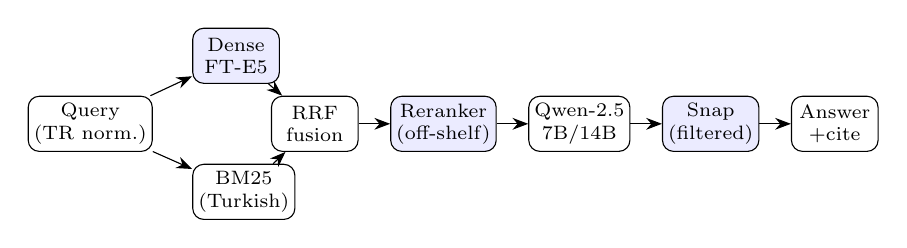
\begin{tikzpicture}[
  font=\scriptsize,
  box/.style={draw, rounded corners, minimum height=7mm, minimum width=11mm,
              align=center, inner sep=2pt},
  ft/.style ={box, fill=blue!8},
  >={Stealth[length=2mm]}, node distance=4.2mm and 4.0mm]
\node[box] (q) {Query\\(TR norm.)};
\node[ft, above right=1.5mm and 5mm of q] (e5) {Dense\\FT-E5};
\node[box, below right=1.5mm and 5mm of q] (bm) {BM25\\(Turkish)};
\node[box, right=15mm of q] (rrf) {RRF\\fusion};
\node[ft, right=4mm of rrf] (rr) {Reranker\\(off-shelf)};
\node[box, right=4mm of rr] (llm) {Qwen-2.5\\7B/14B};
\node[ft, right=4mm of llm] (snap) {Snap\\(filtered)};
\node[box, right=4mm of snap] (ans) {Answer\\+cite};
\draw[->] (q) -- (e5); \draw[->] (q) -- (bm);
\draw[->] (e5) -- (rrf); \draw[->] (bm) -- (rrf);
\draw[->] (rrf) -- (rr); \draw[->] (rr) -- (llm);
\draw[->] (llm) -- (snap); \draw[->] (snap) -- (ans);
\end{tikzpicture}
\caption{Production pipeline. Shaded stages were candidates for domain
adaptation; only the dense encoder's fine-tuning survived ablation (the
reranker is used off-the-shelf; the snap stage is rule-based).}
\label{fig:arch}
\end{figure}

\textbf{Models.} Table~\ref{tab:models} lists the component inventory. A strict
VRAM discipline (one large model resident at a time; explicit cache eviction
between stages) keeps the system within a 16--24\,GB budget; all fine-tuning is
4-bit QLoRA.

\begin{table}[t]
\caption{Model inventory.}
\label{tab:models}
\centering\footnotesize
\begin{tabular}{@{}llll@{}}
\toprule
Model & Params & Role & Adapted \\
\midrule
\texttt{multilingual-e5-large} & 560M & Dense encoder & Yes (FT) \\
\texttt{bge-reranker-v2-m3-tr} & 560M & Cross-encoder & Off-shelf \\
\texttt{Qwen2.5-7B-Instruct}   & 7B   & Generator     & QLoRA (neg.) \\
\texttt{Qwen2.5-14B-Instruct}  & 14B  & Generator (prod.) & No (4-bit) \\
\texttt{bert-...-turkish-nli}  & 110M & Faithfulness  & No \\
\bottomrule
\end{tabular}
\end{table}

%==============================================================================
\section{Methodology}
%==============================================================================
\subsection{Hybrid Retrieval}
Documents are deduplicated and chunked with a legal-aware hierarchical splitter:
first on article boundaries (\texttt{Madde~\textbackslash d+}), then on section
headers (\textsc{B\"{o}l\"{u}m}, \textsc{K\i s\i m}, \textsc{Fas\i l}), then on
paragraph breaks, with recursive character splitting as a fallback. Chunks are
capped at $480$ tokens with $64$-token overlap to respect E5's $512$-token limit
after the \texttt{passage:} prefix. Retrieval spans three sub-corpora: Turkish
Supreme Court (Yarg\i tay) decisions covered lexically by BM25, $45$ statute
codes (\emph{mevzuat}) and a shared legal corpus indexed with both FT-E5 dense
and BM25. Per-source rankings fuse via RRF ($k{=}60$). Turkish-aware
normalization (\.{I}$\to$i, I$\to$\i, etc.) is applied throughout; BM25 uses
whitespace tokenization after stopword removal, since subword tokenization
inflates $n$-gram overlap on agglutinative text.

\subsection{Cross-Encoder Reranking}
The first stage returns up to $50$ candidates per source; a cross-encoder
jointly scores \texttt{[query, passage]} pairs (max length $512$) and the top
$10$ condition the generator. We evaluate two reranker variants: a
domain-fine-tuned cross-encoder (Section~\ref{sec:neg}) and the off-the-shelf
\texttt{bge-reranker-v2-m3} Turkish triplet model; the latter is adopted in
production.

\subsection{Verbatim-Snap Post-Processing}
Triage (Section~\ref{sec:triage}) shows the generator paraphrases away from
source text on a third of questions. The snap post-processor splits retrieved
passages into sentences, scores each by Turkish-normalized token overlap with
the generated answer, and---if the top overlap relative to answer length exceeds
$\tau{=}0.30$---replaces the answer with that verbatim sentence. Crucially,
case-law (Yarg\i tay) passages are filtered from the snap candidate pool: their
decision-style prose matches the statute-formulated gold poorly, and including
them costs $0.0035$ F1.

\subsection{Generation}
The generator uses 4-bit NF4 quantization (double quantization, bfloat16
compute) and greedy decoding (\texttt{temperature}$=0$), which eliminates a
Turkish$\rightarrow$CJK derailment observed under sampling on noisy contexts.
A critical deployment detail: the base 14B model requires
\texttt{repetition\_penalty}$=1.0$; the value $1.2$ tuned for the QLoRA-7B
adapter drives greedy 14B decoding into Chinese mid-sentence on legal contexts.

\subsection{Fine-Tuning Strategies}
\textbf{Embedding.} We built $61$K \texttt{(query, positive, hard-negative)}
triplets, mining hard negatives as high-BM25 passages lacking gold-answer
tokens. Training used a MultipleNegativesRankingLoss (InfoNCE) objective,
effective batch $32$, LR $2{\times}10^{-5}$ cosine, $10$K steps.
\textbf{Reranker.} Fine-tuned on silver \texttt{[query,passage]} pairs labeled
by token overlap with gold (Section~\ref{sec:neg}).
\textbf{Generator.} QLoRA (rank $32$, $\alpha{=}64$, dropout $0.05$, all seven
attention/MLP projections; \texttt{paged\_adamw\_8bit}) on $13.8$K RAG-chat SFT
examples with a strict source-grounding system prompt.

%==============================================================================
\section{Experimental Setup}
%==============================================================================
\subsection{Gold Test Set}
We constructed a $225$-question evaluation set, each entry verified against
official statute text (article number, source code, expected text, provenance),
balanced across five legal domains and three difficulty tiers
(Table~\ref{tab:gold}), and including intentionally unanswerable questions to
test refusal. A cross-LLM audit (five independent verifiers against canonical
\texttt{mevzuat.gov.tr} text) raised verbatim correctness from $91.1\%$ to
$100\%$. The set is evaluation-only; no component is trained on it.

\begin{table}[t]
\caption{Gold set distribution ($225$ questions).}
\label{tab:gold}
\centering\footnotesize
\begin{tabular}{@{}lcccc@{}}
\toprule
Domain & Easy & Medium & Hard & Total \\
\midrule
Criminal / Civil / Commercial & 12 & 18 & 15 & 45 each \\
Administrative / Constitutional & 12 & 18 & 15 & 45 each \\
\midrule
\textbf{Total} & 60 & 90 & 75 & \textbf{225}\\
\bottomrule
\end{tabular}
\end{table}

\subsection{Metrics}
We report \emph{lexical} (Token~F1, ROUGE-L, BLEU), \emph{semantic} (BERTScore-F1
with multilingual BERT), and \emph{retrieval} (Recall@$k$, MRR, nDCG@10) metrics,
all under Turkish-aware normalization. Token~F1 carries bootstrap $95\%$ CIs
($1000$ resamples) and Wilcoxon signed-rank paired tests between configurations.

\textbf{LLM-as-judge.} A judge scores \texttt{(question, gold, prediction,
context)} on correctness, faithfulness, coherence, and relevancy. We hold the
judge model fixed (Qwen-7B) across \emph{all} configurations so comparisons are
apples-to-apples, and we explicitly \emph{validate} it: on a stratified
$30$-question subset, an independent Claude Opus judge agrees on the load-bearing
axes (Spearman $\rho{=}0.72$ correctness, $0.64$ relevancy; both $p{<}0.001$),
preserving the configuration ranking, while revealing that the same-model judge
over-credits correctness by $\approx 0.28$ absolute. We therefore treat absolute
judge scores as upper bounds and rely on the \emph{ranking}.

\textbf{Evaluation scenarios.} Following the course rubric, we compose two
multi-axis scenarios from these metrics: Scenario~2 weights F1\,+\,faithfulness,
Scenario~3 weights correctness\,+\,relevancy\,+\,coherence; Scenario~1 (recall-
weighted) is reported separately in Section~\ref{sec:recall}.

%==============================================================================
\section{Results}
%==============================================================================
Table~\ref{tab:ablation} is the master ablation. Each row adds one component;
the generator-judge is held fixed within the 7B rows so that Phase~6 isolates
the single effect of model scale.

\begin{table*}[t]
\caption{Master ablation on the $225$-question gold set. The generator's
LLM-judge is held fixed (Qwen-7B) across all rows so scoring is comparable;
Phase~6 changes only the generator (7B$\rightarrow$14B). Best per column in
\textbf{bold}.}
\label{tab:ablation}
\centering\footnotesize
\begin{tabular}{@{}llccc c ccc@{}}
\toprule
& \multicolumn{4}{c}{Configuration} & \multicolumn{4}{c}{Metrics}\\
\cmidrule(lr){2-5}\cmidrule(lr){6-9}
ID & Embed & Reranker & Snap & Gen. & Token~F1 [95\% CI] & BERTScore & Judge corr. & Judge faith. \\
\midrule
C1 (Base RAG) & base E5 & --- & --- & 7B & $0.1411$ {\scriptsize[.124,.159]} & $0.6496$ & $0.444$ & --- \\
C2 (+FT embed) & \textbf{FT E5} & --- & --- & 7B & $0.1678$ {\scriptsize[.151,.185]} & $0.6680$ & $0.519$ & --- \\
C3 (+reranker+snap) & FT E5 & off-shelf & Yes & 7B & $0.2386$ & $0.7026$ & $0.736$ & $0.656$ \\
\textbf{Phase 6 (prod.)} & FT E5 & off-shelf & Yes & \textbf{14B} & \best{$0.2648$} {\scriptsize[.243,.288]} & \best{$0.7159$} & \best{$0.750$} & \best{$0.662$} \\
\bottomrule
\end{tabular}
\end{table*}

\textbf{The headline arc.} From the naive baseline to the production system,
Token~F1 rises $0.1411\rightarrow 0.2648$ (\best{$+87.7\%$}); BERTScore
$0.650\rightarrow 0.716$; LLM-judged correctness $0.444\rightarrow 0.750$
($+68.8\%$) and relevancy $0.581\rightarrow 0.849$ ($+46.0\%$). The
single-intervention effect of model scale (C3$\rightarrow$Phase~6) is
$+0.0262$ F1 ($+11.0\%$) with non-overlapping CIs (Phase~6's lower bound
$0.243$ exceeds C3's point estimate $0.239$).

\textbf{Base vs.\ Fine-tuned, same generator.} The rubric asks for a
Base-vs-Fine-tuned comparison holding the LLM constant. Our clean such
comparison is C1 vs.\ C3 (both Qwen-7B): $0.1411\rightarrow 0.2386$, a
$+69.1\%$ relative improvement attributable to retrieval/reranking/post-
processing rather than generator scale. We report the 14B result as a separate
\emph{scaling} axis, not as the fine-tuning contribution, to avoid conflating
the two.

\textbf{Significance and cost.} Wilcoxon paired tests confirm
C1$\rightarrow$C2 ($p{=}0.003$) and C2$\rightarrow$C3 ($p{<}0.001$) on Token~F1;
the C3$\rightarrow$Phase~6 BERTScore CIs are non-overlapping. Inference cost is
$14$\,s/query (7B) to $26$\,s/query (14B) on an L4---well within budget.

%==============================================================================
\section{Component Analysis and Negative Results}
\label{sec:neg}
%==============================================================================
\subsection{Triage Before Tuning}
\label{sec:triage}
Before retraining any component, we bucketed all $225$ questions by whether the
gold content appears in the retrieved context and in the generated answer. The
result reorders priorities: $33\%$ of questions are
\emph{generation-fixable} (gold is in the top-10 context but the model
paraphrases away from it), only $7\%$ are \emph{reranker-fixable}, and $15\%$
are \emph{retrieval-failures}. The generator uses just $37\%$ of the relevant
information retrieval already surfaces (mean answer coverage $0.20$ vs.\ context
coverage $0.54$). This inverts the intuitive assumption that the reranker is the
priority and motivates the snap post-processor and generator scaling.

\subsection{Five Negative Results}
Table~\ref{tab:neg} collects the interventions that \emph{failed}, each with a
transferable cause. We argue these are as informative as the positive results.

\begin{table}[t]
\caption{Negative results. $\Delta$ is Token~F1 vs.\ the relevant comparison
configuration.}
\label{tab:neg}
\centering\footnotesize
\begin{tabular}{@{}lcp{3.2cm}@{}}
\toprule
Intervention & $\Delta$ F1 & Root cause \\
\midrule
Fine-tuned reranker & $\bad\,p{<}.001$ & $52\%$ of training queries had no true-positive passage; silver labels teach an irrelevant-vs-irrelevant distinction. \\
QLoRA (single-pass.) & $-0.065$ & Train (1 passage) / inference ($N$ passages) format mismatch; yet faithfulness $+24$pp. \\
Multi-query (RRF) & $-0.008$ & Paraphrases dilute legal terminology; retrieval drift $>$ fusion gain. \\
HyDE & sanity-fail & Base 7B lacks Turkish-legal knowledge: $5/5$ wrong citations, $1/5$ CJK derail. \\
Citation-snap & $-0.008$ & Brittle to chunk-format noise; oracle headroom only $+0.003$. \\
\bottomrule
\end{tabular}
\end{table}

\textbf{The reranker paradox.} Fine-tuning the cross-encoder degraded F1 in
every configuration (e.g., adding it to FT-embed dropped $0.168\rightarrow
0.126$; Wilcoxon $p{<}0.001$), whereas the off-the-shelf reranker lifted F1 to
$0.239$. Post-hoc analysis found $52\%$ of training queries had no genuinely
relevant passage in the corpus, so silver labeling taught the model to rank one
irrelevant passage over another---corrupting its pretrained signal.

\textbf{The QLoRA paradox.} The QLoRA generator \emph{succeeded at its
behavioral target}---faithfulness rose $0.43\rightarrow 0.67$ ($+24$pp) and
citation emission appeared for the first time---yet Token~F1 \emph{fell}
$0.065$. The cause is a train/inference shape mismatch: the SFT data presented a
single passage (\texttt{[Kaynak]\textbackslash nMetin:...}) whereas inference
concatenates many (\texttt{[Kaynak 1]...[Kaynak N]}); the model anchored to the
wrong passage. This decoupling of behavioral success from metric regression is,
we argue, the report's most interesting finding about RAG fine-tuning.

\textbf{Prompt design exceeds model fine-tuning.} Standardizing the system
prompt alone improved the baseline $0.0950\rightarrow 0.1411$ ($+49\%$),
exceeding any single component fine-tuning; conversely, four ``stricter''
extractive prompts all \emph{hurt} (down to $0.135$) via over-refusal and
citation-token noise. The leverage is in what the model was trained on, not how
it is constrained at inference.

%==============================================================================
\section{Faithfulness and Hallucination}
%==============================================================================
We measure faithfulness with a Turkish NLI sentence encoder: each answer
sentence is scored by its maximum similarity to any retrieved-context sentence;
sentences below $0.50$ are flagged as hallucinated. On the production
(Phase~6) system, mean NLI faithfulness is $0.765$ and the hallucination rate
is $\best{8.95\%}$---roughly half the $17.0\%$ of the 7B configuration. The
difficulty gradient persists but flattens: hard questions hallucinate at
$18.8\%$ versus $\sim\!4\%$ for easy/medium (Table~\ref{tab:halluc}), down from
$31.9\%$ at 7B. By domain, administrative answers are most faithful
($0.83$, $5.5\%$) and criminal/constitutional least ($12.6\%$)---consistent with
the 7B pattern at roughly half the absolute rate. The $32\%$-on-hard signal
motivating difficulty-aware abstention is materially mitigated by scale.

\begin{table}[t]
\caption{Phase-6 hallucination by difficulty (NLI, threshold $0.50$).}
\label{tab:halluc}
\centering\footnotesize
\begin{tabular}{@{}lccc@{}}
\toprule
Difficulty & NLI faithfulness & Halluc.\ rate & Token~F1 \\
\midrule
Easy & $0.797$ & $4.3\%$ & $0.298$ \\
Medium & $0.790$ & $3.5\%$ & $0.279$ \\
Hard & $0.710$ & $18.8\%$ & $0.218$ \\
\midrule
\textbf{Overall} & \textbf{0.765} & \textbf{8.95\%} & $0.265$ \\
\bottomrule
\end{tabular}
\end{table}

%==============================================================================
\section{Retrieval Evaluation (Scenario 1)}
\label{sec:recall}
%==============================================================================
Our progress report could only report \emph{proxy} relevance (token overlap),
which paradoxically favored the \emph{base} encoder---an artifact we now
explain: contrastive fine-tuning optimizes for \emph{semantic} retrieval
utility (passages that help the model reason) rather than answer-extractive
overlap, so a token-overlap proxy systematically undervalues it. With a
chunk-labeled benchmark ($240$ questions, gold passage IDs), the production
retrieval stack (3-corpus FT-E5\,+\,BM25\,+\,off-shelf reranker) attains
Recall@5 $0.854$, \best{Recall@10 $0.875$}, MRR $0.770$, nDCG@10 $0.796$---up
from $0.79$ Recall@10 for the dense-only baseline.

\noindent\emph{Honest caveat.} This benchmark is a course-provided set, not the
held-out evaluation, and is plausibly in-distribution for our fine-tuned
encoder; we therefore treat its recall as an \emph{upper bound}, not a
prediction of held-out performance. The value of this number is as evidence
that the retrieval machinery and our metric pipeline are sound---and the
deployed system computes the same metric on any evaluator-supplied benchmark
(Section~\ref{sec:deploy}).

%==============================================================================
\section{Deployment and Robustness}
\label{sec:deploy}
%==============================================================================
Because the held-out evaluation runs on documents and questions unseen by any
team, robustness to arbitrary inputs---not a higher score on a self-chosen
set---is the operative goal. The system exposes a CLI
(\texttt{ingest}/\texttt{benchmark}/\texttt{query}) that (i)~ingests raw
directories of PDF/text or pre-chunked JSONL, building FAISS\,+\,BM25 indexes
(with an exact \texttt{IndexFlatIP} fallback for small corpora); (ii)~parses
benchmarks in Turkish (\texttt{\{soru, cevap, ilgili\_belgeler\}}) or English
schemas; and (iii)~auto-selects \emph{document-level} Recall@$k$ when a
benchmark labels relevance by document rather than by our internal chunk IDs
(which are freshly minted per ingest and therefore never match external labels).

We validate this end to end: ingesting three previously unseen statute PDFs and
running the production configuration on a hand-written Turkish benchmark yields
document-level Recall@10 $=1.0$, zero language derailment, and coherent Turkish
answers (one verbatim-snapping a statute article, one correctly abstaining).
This confirms the pipeline satisfies the ``bring-your-own-data'' requirement
with the full metric suite intact.

%==============================================================================
\section{Discussion and Limitations}
%==============================================================================
\textbf{Adaptation $\neq$ fine-tuning.} Our strongest single lever was model
scale (7B$\rightarrow$14B), which is \emph{not} domain adaptation; among genuine
fine-tuning interventions only the embedding encoder helped. We report these
honestly rather than packaging scale as a fine-tuning win.

\textbf{Self-reported numbers are evidence, not predictions.} The gold and
shared sets measure methodology and system quality; the graded evaluation is on
unseen data. We designed for that uncertainty (Section~\ref{sec:deploy}).

\textbf{Open limitations.} (i)~Corpus gaps: the constitutional domain is
under-covered (the case-law corpus is Supreme-Court-centric), the dominant
retrieval-failure source. (ii)~The QLoRA format mismatch is fixable by training
on multi-passage data, which would likely convert the $+24$pp faithfulness gain
into a Token~F1 gain. (iii)~On the most recent Colab image, the updated
\texttt{transformers} loader materializes fp16 shards before quantizing, so 14B
OOMs a $22$\,GB GPU at load; the 7B production configuration is the robust
default, and the 14B headline stands from a run on the prior stack.

%==============================================================================
\section{Conclusion}
%==============================================================================
We built a Turkish-legal RAG pipeline that improves a naive baseline by
$+87.7\%$ Token~F1 and halves hallucination, and---through a triage-driven,
negative-result-forward methodology---showed \emph{which} adaptations actually
pay off. The decisive gains came from off-the-shelf components, a rule-based
post-processor, and model scale; our fine-tuned reranker and QLoRA generator
both regressed, each for an instructive and transferable reason. Future work:
retrain QLoRA on multi-passage data to realize its latent faithfulness gain,
close the constitutional-corpus gap, and map the reranker label-noise tolerance
curve.

%==============================================================================
\begin{thebibliography}{99}
\footnotesize
\bibitem{lewis2020rag} P.~Lewis \emph{et al.}, ``Retrieval-Augmented Generation
for Knowledge-Intensive NLP Tasks,'' \emph{NeurIPS}, 2020.
\bibitem{wang2024e5} L.~Wang \emph{et al.}, ``Text Embeddings by
Weakly-Supervised Contrastive Pre-training,'' \emph{ACL}, 2024.
\bibitem{robertson2009bm25} S.~Robertson and H.~Zaragoza, ``The Probabilistic
Relevance Framework: BM25 and Beyond,'' \emph{Found.\ Trends IR}, 3(4), 2009.
\bibitem{cormack2009rrf} G.~Cormack, C.~Clarke, and S.~Buettcher, ``Reciprocal
Rank Fusion Outperforms Condorcet and Individual Rank Learning Methods,''
\emph{SIGIR}, 2009.
\bibitem{johnson2019faiss} J.~Johnson, M.~Douze, and H.~J\'egou, ``Billion-Scale
Similarity Search with GPUs,'' \emph{IEEE Trans.\ Big Data}, 7(3), 2019.
\bibitem{hu2022lora} E.~J.~Hu \emph{et al.}, ``LoRA: Low-Rank Adaptation of Large
Language Models,'' \emph{ICLR}, 2022.
\bibitem{dettmers2023qlora} T.~Dettmers \emph{et al.}, ``QLoRA: Efficient
Finetuning of Quantized LLMs,'' \emph{NeurIPS}, 2023.
\bibitem{gao2023hyde} L.~Gao \emph{et al.}, ``Precise Zero-Shot Dense Retrieval
without Relevance Labels,'' \emph{ACL}, 2023.
\bibitem{asai2024selfrag} A.~Asai \emph{et al.}, ``Self-RAG: Learning to
Retrieve, Generate, and Critique through Self-Reflection,'' \emph{ICLR}, 2024.
\bibitem{zhang2020bertscore} T.~Zhang \emph{et al.}, ``BERTScore: Evaluating Text
Generation with BERT,'' \emph{ICLR}, 2020.
\bibitem{zheng2023judge} L.~Zheng \emph{et al.}, ``Judging LLM-as-a-Judge with
MT-Bench and Chatbot Arena,'' \emph{NeurIPS}, 2023.
\bibitem{turknli2024} ``legal\_nli\_TR\_V1: Turkish Commercial Court NLI
Dataset,'' HuggingFace Datasets, 2024.
\bibitem{qwen2024} Qwen Team, ``Qwen2.5 Technical Report,'' 2024.
\end{thebibliography}

\end{document}
